\documentclass[landscape,a0b,final]{a0poster}
\usepackage{german}
\usepackage{amssymb}
\usepackage{tikz}
\usepackage{type1cm}
\begin{document}
\begin{center}

\end{center}
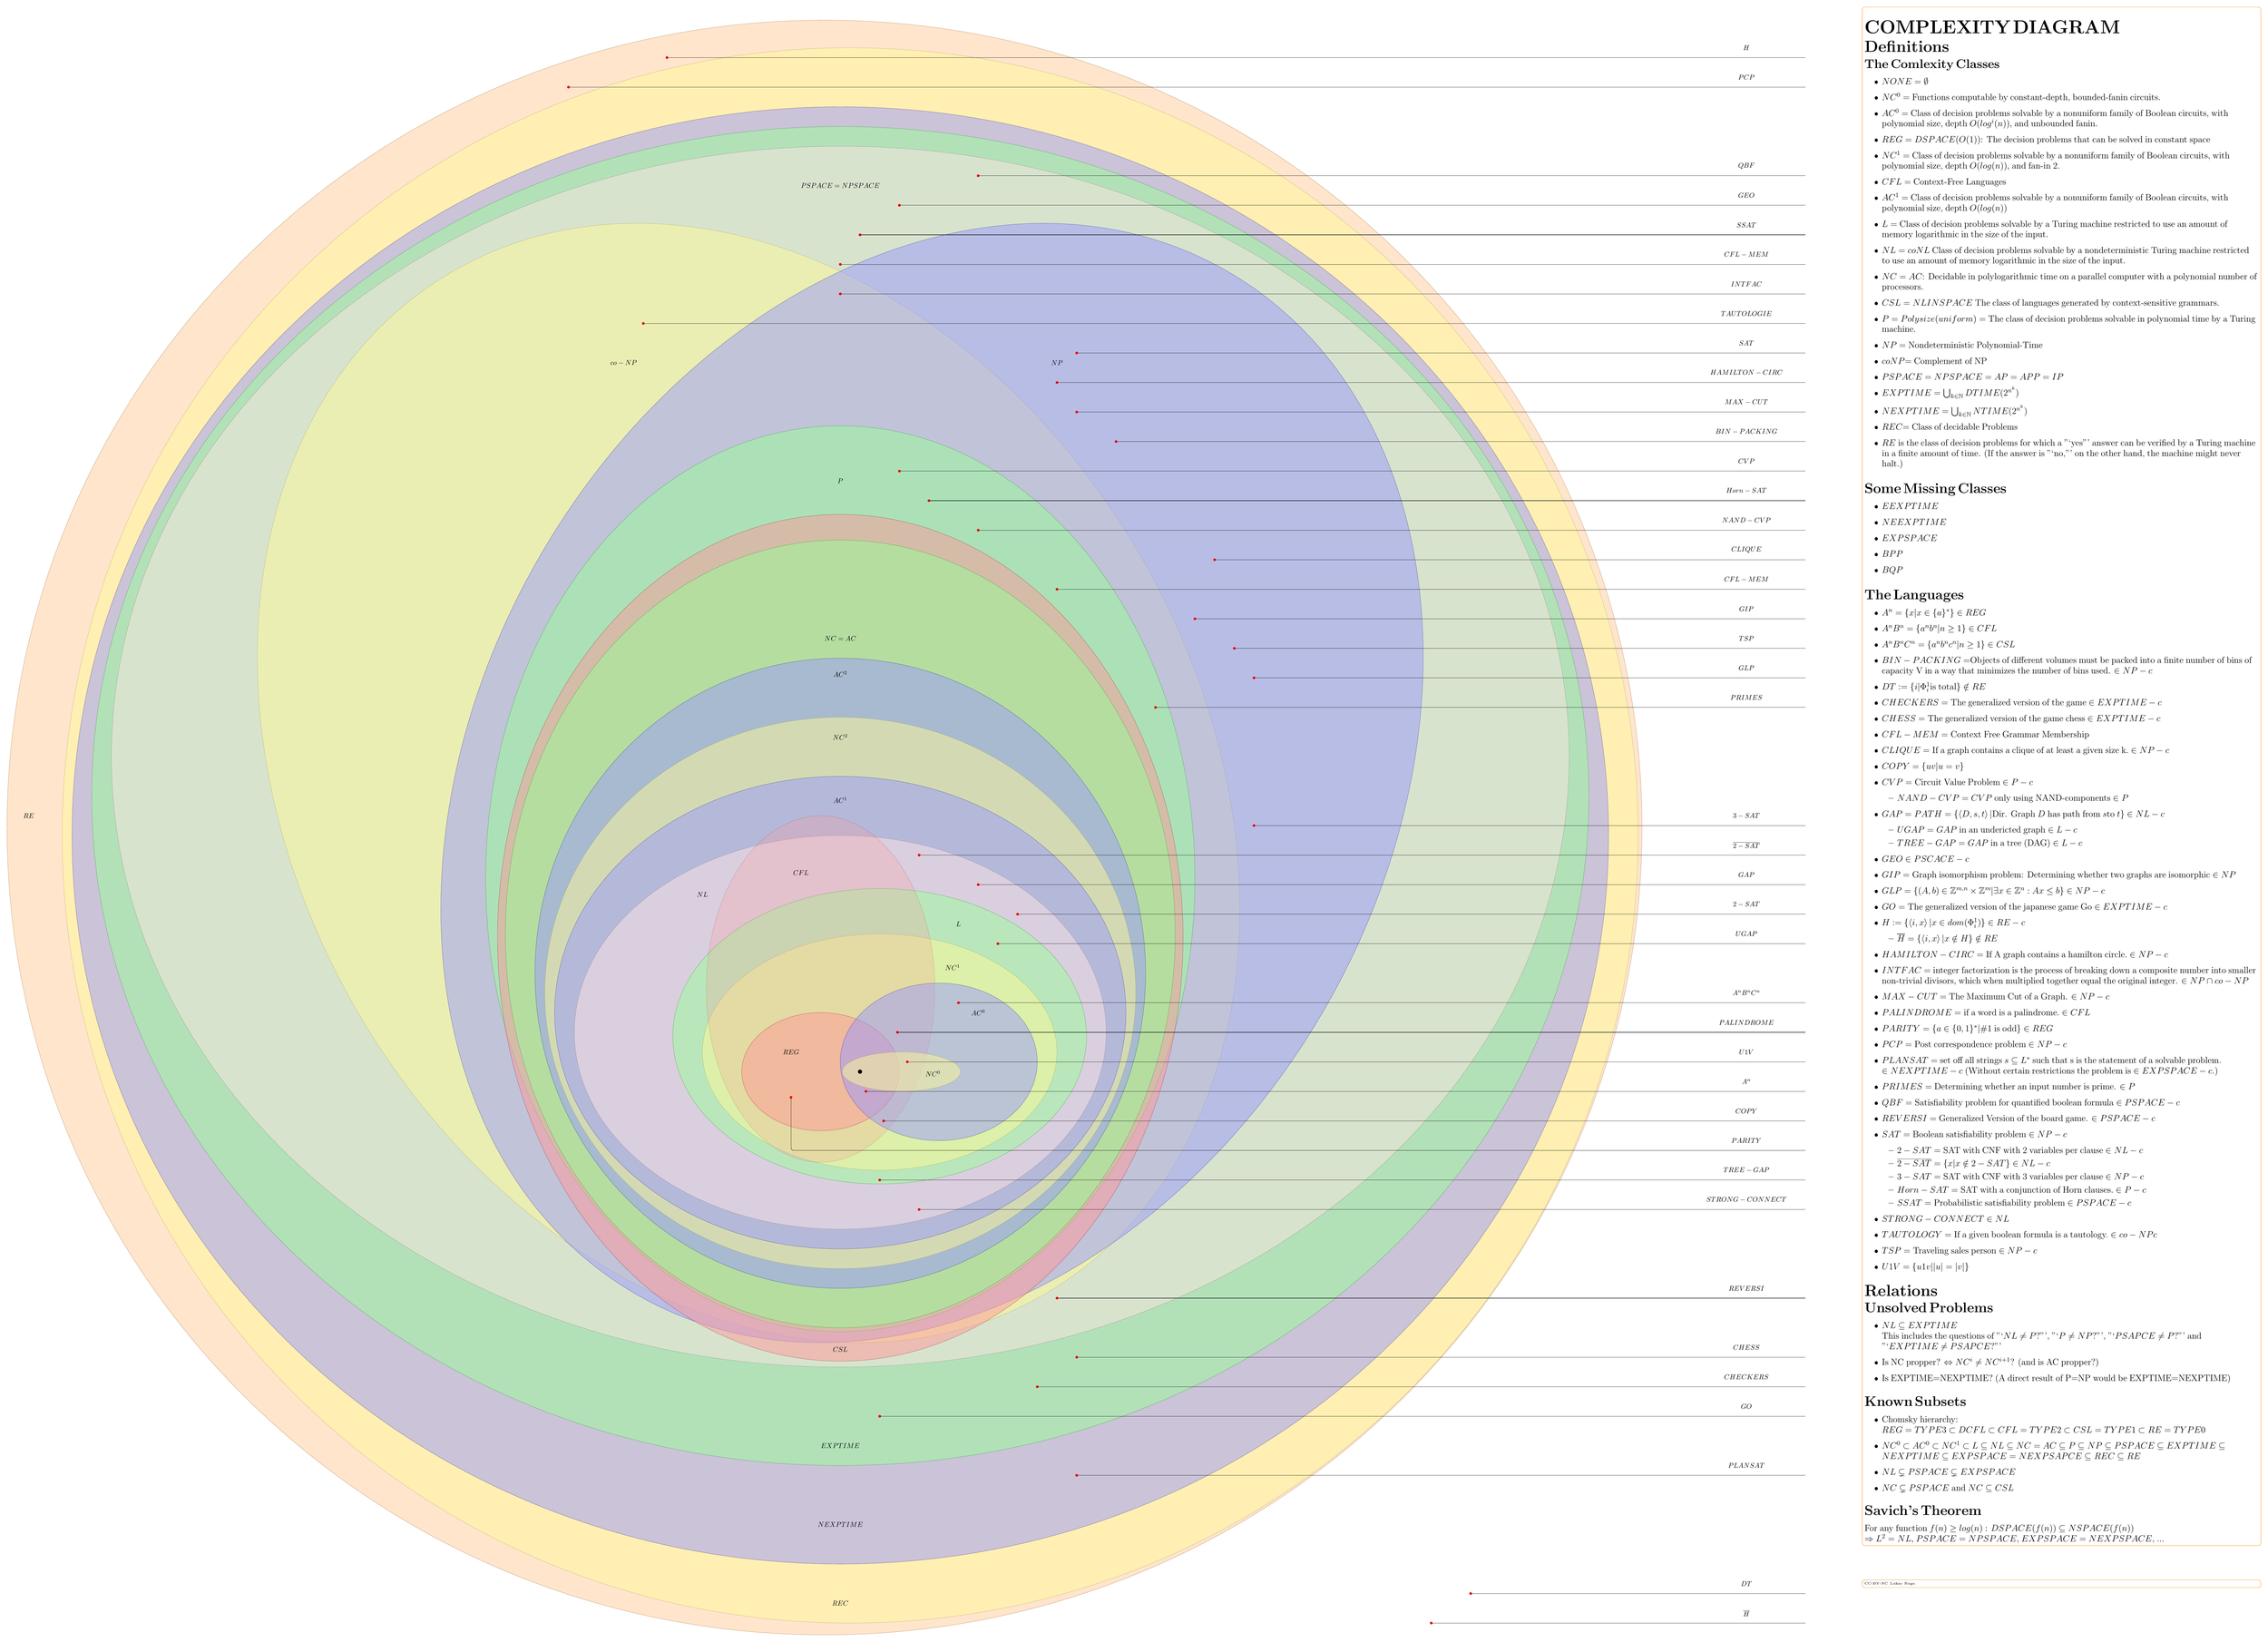
\begin{tikzpicture}[rounded corners]
%\draw (-51,0) -- (51,0);
%\draw (0,-42) -- (0,42);
%Die Komplexit�tsklassen
%RE
\filldraw[fill=orange!40!white, draw=orange!50!black, semitransparent] (-0.8,4.4) ellipse (41.5cm and 41cm);
\draw (-41.2,5) node {\(RE\)};
%REC
\filldraw[fill=yellow!40!white, draw=yellow!50!black, semitransparent] (0.5,4) ellipse (40cm and 40cm);
\draw (0,-35) node {\(REC\)};
%NEXPTIME
\filldraw[fill=blue!40!white, draw=blue!50!black, semitransparent] (0,4) ellipse (39cm and 37cm);
\draw (0,-31) node {\(NEXPTIME\)};
%EXPTIME
\filldraw[fill=green!40!white, draw=green!50!black, semitransparent] (0,6) ellipse (38cm and 34cm);
\draw (0,-27) node {\(EXPTIME\)};
%PSPACE
\filldraw[fill=pink!40!white, draw=pink!50!black, semitransparent] (0,8) ellipse (37cm and 31cm);
\draw (0,37) node {\(PSPACE=NPSPACE\)};
%Co-NP
\filldraw[fill=yellow!40!white, draw=yellow!50!black, semitransparent][rotate=-60] (-8.1,-0.7) ellipse (30cm and 23cm);
\draw (-11,28) node {\(co-NP\)};
%NP
\filldraw[fill=blue!40!white, draw=blue!50!black, semitransparent][rotate=60] (8.1,-0.7) ellipse (30cm and 23cm);
\draw (11,28) node {\(NP\)};
%P
\filldraw[fill=green!40!white, draw=green!50!black, semitransparent] (0,1.8) ellipse (18cm and 23cm);
\draw (0,22) node {\(P\)};
%CSL
\filldraw[fill=red!40!white, draw=red!50!black, semitransparent] (0,-1.2) ellipse (17.4cm and 21.5cm);
\draw (0,-22.1) node {\(CSL\)};
%NC=AC
\filldraw[fill=green!40!white, draw=green!50!black, semitransparent] (0,-1) ellipse (17cm and 20cm);
\draw (0,14) node {\(NC=AC\)};
%AC2
\filldraw[fill=blue!40!white, draw=blue!50!black, semitransparent] (0,-3) ellipse (15.5cm and 16cm);
\draw (0,12.2) node {\(AC^2\)};
%NC2
\filldraw[fill=yellow!40!white, draw=yellow!50!black, semitransparent] (0,-4) ellipse (15cm and 14cm);
\draw (0,9) node {\(NC^2\)};
%AC1
\filldraw[fill=blue!40!white, draw=blue!50!black, semitransparent] (0,-5) ellipse (14.5cm and 12cm);
\draw (0,5.8) node {\(AC^1\)};
%NL
\filldraw[fill=pink!40!white, draw=pink!50!black, semitransparent] (0,-6) ellipse (13.5cm and 10cm);
\draw (-7,1) node {\(NL\)};
%L
\filldraw[fill=green!40!white, draw=green!50!black, semitransparent] (2,-6.2) ellipse (10.5cm and 7.5cm);
\draw (6,-0.5) node {\(L\)};
%NC1
\filldraw[fill=yellow!40!white, draw=yellow!50!black, semitransparent] (2,-7) ellipse (9cm and 6cm);
\draw (5.7,-2.7) node {\(NC^1\)};
%CFL
\filldraw[fill=red!40!white, draw=red!50!black, nearly transparent] (-1,-3.8) ellipse (5.8cm and 8.8cm);
\draw (-2,2.1) node {\(CFL\)};
%REG
\filldraw[fill=red!40!white, draw=red!50!black, semitransparent] (-1,-8) ellipse (4cm and 3cm);
\draw (-2.5,-7) node {\(REG\)};
%AC0
\filldraw[fill=blue!40!white, draw=blue!50!black, semitransparent] (5,-7.5) ellipse (5cm and 4cm);
\draw (7,-5) node {\(AC^0\)};
%NC0
\filldraw[fill=yellow!40!white, draw=yellow!50!black, semitransparent] (3.1,-8) ellipse (3cm and 1cm);
\draw (4.7,-8.1) node {\(NC^0\)};
%NONE
%TC0
%blablablablablabla irgendwo
\fill[black] (1,-8) circle (3pt);
% Die Sprachen/Probleme
%Rechts Oben
%H
\fill[red] (-8.8,43.5) circle (2pt);
\draw (-8.8,43.5)--(49,43.5);
\draw (46,44) node {\(H\)};
%PCP
\fill[red] (-13.8,42) circle (2pt);
\draw (-13.8,42)--(49,42);
\draw (46,42.5) node {\(PCP\)};
%QBF
\fill[red] (7,37.5) circle (2pt);
\draw (7,37.5)--(49,37.5);
\draw (46,38) node {\(QBF\)};
%GEO
\fill[red] (3,36) circle (2pt);
\draw (3,36)--(49,36);
\draw (46,36.5) node {\(GEO\)};
%SSAT
\fill[red] (1,34.5) circle (2pt);
\draw (1,34.5)--(49,34.5);
\draw (46,35) node {\(SSAT\)};
%CFL-MEM
\fill[red] (0,33) circle (2pt);
\draw (0,33)--(49,33);
\draw (46,33.5) node {\(CFL-MEM\)};
%INTFAC
\fill[red] (0,31.5) circle (2pt);
\draw (0,31.5)--(49,31.5);
\draw (46,32) node {\(INTFAC\)};
%TAUTOLOGIE
\fill[red] (-10,30) circle (2pt);
\draw (-10,30)--(49,30);
\draw (46,30.5) node {\(TAUTOLOGIE\)};
%SAT
\fill[red] (12,28.5) circle (2pt);
\draw (12,28.5)--(49,28.5);
\draw (46,29) node {\(SAT\)};
%HAMILTON-CIRC
\fill[red] (11,27) circle (2pt);
\draw (11,27)--(49,27);
\draw (46,27.5) node {\(HAMILTON-CIRC\)};
%MAX-CUT
\fill[red] (12,25.5) circle (2pt);
\draw (12,25.5)--(49,25.5);
\draw (46,26) node {\(MAX-CUT\)};
%BIN-PACKING
\fill[red] (14,24) circle (2pt);
\draw (14,24)--(49,24);
\draw (46,24.5) node {\(BIN-PACKING\)};
%CVP
\fill[red] (3,22.5) circle (2pt);
\draw (3,22.5)--(49,22.5);
\draw (46,23) node {\(CVP\)};
%Horn-SAT
\fill[red] (4.5,21) circle (2pt);
\draw (4.5,21)--(49,21);
\draw (46,21.5) node {\(Horn-SAT\)};
%NAND-CVP
\fill[red] (7,19.5) circle (2pt);
\draw (7,19.5)--(49,19.5);
\draw (46,20) node {\(NAND-CVP\)};
%CLIQUE
\fill[red] (19,18) circle (2pt);
\draw (19,18)--(49,18);
\draw (46,18.5) node {\(CLIQUE\)};
%Context Free Grammar Membership
\fill[red] (11,16.5) circle (2pt);
\draw (11,16.5)--(49,16.5);
\draw (46,17) node {\(CFL-MEM\)};
%graph isomorphism problem
\fill[red] (18,15) circle (2pt);
\draw (18,15)--(49,15);
\draw (46,15.5) node {\(GIP\)};
%TSP
\fill[red] (20,13.5) circle (2pt);
\draw (20,13.5)--(49,13.5);
\draw (46,14) node {\(TSP\)};
%GLP
\fill[red] (21,12) circle (2pt);
\draw (21,12)--(49,12);
\draw (46,12.5) node {\(GLP\)};
%PRIMES
\fill[red] (16,10.5) circle (2pt);
\draw (16,10.5)--(49,10.5);
\draw (46,11) node {\(PRIMES\)};
%3-SAT
\fill[red] (21,4.5) circle (2pt);
\draw (21,4.5)--(49,4.5);
\draw (46,5) node {\(3-SAT\)};
%nicht2SAT
\fill[red] (4,3) circle (2pt);
\draw (4,3)--(49,3);
\draw (46,3.5) node {\(\overline{2-SAT}\)};
%GAP
\fill[red] (7,1.5) circle (2pt);
\draw (7,1.5)--(49,1.5);
\draw (46,2) node {\(GAP\)};
%2-SAT
\fill[red] (9,0) circle (2pt);
\draw (9,0)--(49,0);
\draw (46,0.5) node {\(2-SAT\)};
%UGAP
\fill[red] (8,-1.5) circle (2pt);
\draw (8,-1.5)--(49,-1.5);
\draw (46,-1) node {\(UGAP\)};
%AnBnCn
\fill[red] (6,-4.5) circle (2pt);
\draw (6,-4.5)--(49,-4.5);
\draw (46,-4) node {\(A^nB^nC^n\)};
%PALINDROME
\fill[red] (2.9,-6) circle (2pt);
\draw (2.9,-6)--(49,-6);
\draw (46,-5.5) node {\(PALINDROME\)};
%U1V
\fill[red] (3.4,-7.5) circle (2pt);
\draw (3.4,-7.5)--(49,-7.5);
\draw (46,-7) node {\(U1V\)};
%A^n
\fill[red] (1.3,-9) circle (2pt);
\draw (1.3,-9)--(49,-9);
\draw (46,-8.5) node {\(A^n\)};
%COPY
\fill[red] (2.2,-10.5) circle (2pt);
\draw (2.2,-10.5)--(49,-10.5);
\draw (46,-10) node {\(COPY\)};
%PARITY
\fill[red] (-2.5,-9.3) circle (2pt);
\draw (-2.5,-9.3)--(-2.5,-12)--(49,-12);
\draw (46,-11.5) node {\(PARITY\)};
%TREE-GAP
\fill[red] (2,-13.5) circle (2pt);
\draw (2,-13.5)--(49,-13.5);
\draw (46,-13) node {\(TREE-GAP\)};
%STRONG-CONNECT
\fill[red] (4,-15) circle (2pt);
\draw (4,-15)--(49,-15);
\draw (46,-14.5) node {\(STRONG-CONNECT\)};
%Reversi
\fill[red] (11,-19.5) circle (2pt);
\draw (11,-19.5)--(49,-19.5);
\draw (46,-19) node {\(REVERSI\)};
%CHESS
\fill[red] (12,-22.5) circle (2pt);
\draw (12,-22.5)--(49,-22.5);
\draw (46,-22) node {\(CHESS\)};
%checkers
\fill[red] (10,-24) circle (2pt);
\draw (10,-24)--(49,-24);
\draw (46,-23.5) node {\(CHECKERS\)};
%GO
\fill[red] (2,-25.5) circle (2pt);
\draw (2,-25.5)--(49,-25.5);
\draw (46,-25) node {\(GO\)};
%PLANSAT
\fill[red] (12,-28.5) circle (2pt);
\draw (12,-28.5)--(49,-28.5);
\draw (46,-28) node {\(PLANSAT\)};
%DT
\fill[red] (32,-34.5) circle (2pt);
\draw (32,-34.5)--(49,-34.5);
\draw (46,-34) node {\(DT\)};
%nichtH
\fill[red] (30,-36) circle (2pt);
\draw (30,-36)--(49,-36);
\draw (46,-35.5) node {\(\overline{H}\)};
%Legend
\draw (62,7) node[fill=white,text width=20cm, draw=orange]
{\section*{\fontsize{27}{15}\selectfont COMPLEXITY DIAGRAM}
\fontsize{13}{15}\selectfont
\subsection*{\fontsize{23}{15}\selectfont Definitions}
\subsubsection*{\fontsize{18}{15}\selectfont The Comlexity Classes}
	\begin{itemize}
		\item \(NONE=\emptyset \)
		\item \(NC^0=\) Functions computable by constant-depth, bounded-fanin circuits.
		\item \(AC^0=\) Class of decision problems solvable by a nonuniform family of Boolean circuits, with polynomial size, depth \(O(log^i(n))\), and unbounded fanin.
		\item \(REG=DSPACE(O(1))\): The decision problems that can be solved in constant space
		\item \(NC^1=\) Class of decision problems solvable by a nonuniform family of Boolean circuits, with polynomial size, depth \(O(log(n))\), and fan-in \(2\).
		\item \(CFL=\) Context-Free Languages 
		\item \(AC^1=\) Class of decision problems solvable by a nonuniform family of Boolean circuits, with polynomial size, depth \(O(log(n))\)
		\item \(L=\) Class of decision problems solvable by a Turing machine restricted to use an amount of memory logarithmic in the size of the input.
		\item \(NL=coNL\) Class of decision problems solvable by a nondeterministic Turing machine restricted to use an amount of memory logarithmic in the size of the input. 
		\item \(NC=AC\): Decidable in polylogarithmic time on a parallel computer with a polynomial number of processors.
		\item  \(CSL = NLINSPACE\) The class of languages generated by context-sensitive grammars. 
		\item \(P=Polysize (uniform) =\) The class of decision problems solvable in polynomial time by a Turing machine.
		\item \(NP\) = Nondeterministic Polynomial-Time 
		\item \(coNP\)=  Complement of NP
		\item \(PSPACE=NPSPACE=AP=APP=IP\)
		\item \(EXPTIME = \bigcup_{k\in \mathbb{N}} DTIME (2^{n^k})\)
		\item \(NEXPTIME = \bigcup_{k\in \mathbb{N}} NTIME (2^{n^k})\)
		\item \(REC\)= Class of decidable Problems
		\item \(RE\) is the class of decision problems for which a "`yes"' answer can be verified by a Turing machine in a finite amount of time. (If the answer is "`no,"' on the other hand, the machine might never halt.)
	\end{itemize}
\subsubsection*{\fontsize{20}{20}\selectfont Some Missing Classes}
\begin{itemize}
	\item \(EEXPTIME\)
	\item \(NEEXPTIME\)
	\item \(EXPSPACE\)
	\item \(BPP\)
	\item \(BQP\)
\end{itemize}
\subsubsection*{\fontsize{20}{20}\selectfont The Languages}
	\begin{itemize}
		\item \(A^n=\{x | x \in \{a\}^*\}\in REG\)
		\item \(A^nB^n=\{a^nb^n | n \geq 1\}\in CFL\)
		\item \(A^nB^nC^n=\{a^nb^nc^n | n \geq 1\}\in CSL\)
		\item \(BIN-PACKING=\)Objects of different volumes must be packed into a finite number of bins of capacity V in a way that minimizes the number of bins used. \(\in NP-c\)
		\item \(DT:=\{i|\Phi_i^1 \mbox{is total}\} \notin RE\)
		\item \(CHECKERS=\mbox{The generalized version of the game}\in EXPTIME-c\)
		\item \(CHESS=\mbox{The generalized version of the game chess}\in EXPTIME-c\)
		\item \(CFL-MEM =\mbox{Context Free Grammar Membership} \)
		\item \(CLIQUE=\mbox{If a graph contains a clique of at least a given size k.} \in NP-c\)
		\item \(COPY= \{ uv | u=v\}\)
		\item \(CVP=\mbox{Circuit Value Problem} \in P-c\)
		\begin{itemize}
			\item \(NAND-CVP=CVP \mbox{ only using NAND-components} \in P\)
		\end{itemize}
		\item\(GAP=PATH=\{\left\langle D, s, t\right\rangle |\mbox{Dir. Graph } D \mbox{ has path from } s \mbox {to } t\} \in NL-c\)
		\begin{itemize}
			\item\(UGAP= GAP\mbox{ in an undericted graph} \in L-c\)
			\item\(TREE-GAP=GAP \mbox{ in a tree (DAG)} \in L-c\)
		\end{itemize}
		\item\(GEO \in PSCACE-c\)
		\item \(GIP=\mbox{Graph isomorphism problem: Determining whether two graphs are isomorphic} \in NP \) 
		\item\(GLP=\{(A,b) \in \mathbb{Z}^{m,n}\times \mathbb{Z}^{m} | \exists x \in \mathbb{Z}^{n}: Ax \leq b\} \in NP-c\)
		\item \(GO=\mbox{The generalized version of the japanese game Go} \in EXPTIME-c \)
		\item \(H:=\{\left\langle i,x\right\rangle | x \in dom(\Phi_i^1)\} \in RE-c\)
		\begin{itemize}
				\item \(\overline{H}=\{\left\langle i,x\right\rangle | x \notin H\} \notin RE\)
			\end{itemize}
		\item \(HAMILTON-CIRC=\mbox{If A graph contains a hamilton circle.} \in NP-c\)
		\item \(INTFAC=\) integer factorization is the process of breaking down a composite number into smaller non-trivial divisors, which when multiplied together equal the original integer. \(\in NP \cap co-NP\)
		\item \(MAX-CUT = \) The Maximum Cut of a Graph. \(\in NP-c\) 
		\item \(PALINDROME=\mbox{if a word is a palindrome.} \in CFL\)
		\item \(PARITY=\{a\in\{0,1\}^*| \#1 \mbox{ is odd}\} \in REG\)
		\item \(PCP=\mbox{Post correspondence problem}\in NP-c\)
		\item \(PLANSAT=\) set off all strings \(s\subseteq L^*\) such that s is the statement of a solvable problem. \(\in NEXPTIME-c\) (Without certain restrictions the problem is \(\in EXPSPACE-c\).)
		\item \(PRIMES=\) Determining whether an input number is prime. \(\in P\)
		\item \(QBF=\mbox{Satisfiability problem for quantified boolean formula} \in PSPACE-c\)
		\item \(REVERSI=\) Generalized Version of the board game. \(\in PSPACE-c\)
		\item \(SAT=\mbox{Boolean satisfiability problem}\in NP-c\)
		\begin{itemize}
			\item \(2-SAT=\mbox{SAT with CNF with 2 variables per clause}\in NL-c\)
			\item \(\overline{2-SAT}=\{x|x \notin 2-SAT\} \in NL-c\)
			\item \(3-SAT=\mbox{SAT with CNF with 3 variables per clause} \in NP-c\)
			\item \(Horn-SAT=\mbox{SAT with a conjunction of Horn clauses.} \in P-c\)
			\item\(SSAT = \mbox{Probabilistic satisfiability problem}\in PSPACE-c\)
		\end{itemize}
		\item\(STRONG-CONNECT\in NL\)
		\item \(TAUTOLOGY=\mbox{If a given boolean formula is a tautology.} \in co-NPc\)
		\item \(TSP=\mbox{Traveling sales person} \in NP-c \)
		\item \(U1V = \{ u1v | |u|=|v| \} \)
	\end{itemize}
\subsection*{\fontsize{23}{15}\selectfont Relations}
\subsubsection*{\fontsize{20}{15}\selectfont Unsolved Problems}
\begin{itemize}
\item \(NL \subseteq EXPTIME\)\\
This includes the questions of "`\(NL \neq P\)?"', "`\(P \neq NP\)?"', "`\(PSAPCE \neq P\)?"' and "`\(EXPTIME \neq PSAPCE\)?"'
\item Is NC propper? \(\Leftrightarrow\) \(NC^i \neq NC^{i+1}\)? (and is AC propper?)
\item Is EXPTIME=NEXPTIME? (A direct result of P=NP would be EXPTIME=NEXPTIME)
\end{itemize}
\subsubsection*{\fontsize{20}{15}\selectfont Known Subsets}
\begin{itemize}
\item Chomsky hierarchy: \(REG=TYPE3 \subset DCFL \subset CFL=TYPE2 \subset CSL=TYPE1 \subset RE=TYPE0\) \\
\item \(NC^0 \subset AC^0 \subset NC^1 \subset L \subseteq NL \subseteq NC=AC \subseteq P \subseteq NP \subseteq PSPACE \subseteq EXPTIME \subseteq NEXPTIME \subseteq EXPSPACE=NEXPSAPCE \subseteq REC \subseteq RE\)
\item \(NL \subsetneq PSPACE \subsetneq EXPSPACE\) \\
\item \( NC \subsetneq PSPACE\) and \(NC \subseteq CSL\) \\
\end{itemize}
\subsubsection*{\fontsize{20}{15}\selectfont Savich's Theorem}

For any function \(f(n) \geq log(n) \) : \(DSPACE(f(n)) \subseteq NSPACE(f(n)) \) \\
\(\Rightarrow \) \(L^2 = NL\), \(PSPACE = NPSPACE\), \(EXPSPACE=NEXPSPACE\), ...\\
};
\draw (62,-34) node[fill=white,text width=20cm, draw=orange]
{
\tiny
CC-BY-NC Lukas Ruge.
};
\end{tikzpicture}
\end{document}